\newchapt{Tapered Structure Detection}{chapt6}{Tapered Structure Detection}

After the keyslices are detected and vectorized, the contours of
$N_K = \{I_{i}, i = 0, ..., K \}$ keyslices are used to represent
the building based on the extrusion operation.
That is, the space between each pair of keyslices, say $I_{i}$ and $I_{j}$,
can be interpolated by the lower keyslice, e.g., $I_{i}$ in this case.
This is valid due to the similarity between the intermediate slices
and the keyslice $I_{i}$.
By modeling a building using this series of keyslices $N_K$, we
significantly reduce the polygon count for urban buildings. 
An example of the reconstructed model is shown in \Fig{DXF_notaper_model}.
This helps make possible 3D web-based applications such as 3D city navigation.

In addition to the extrusion operation, we can further improve the model
and reduce the model size by observing that part of the keyslice images
belong to the same tapered structure, as demonstrated in \Fig{DXF_top}.
\Figa{DXF_top} shows the roof structure
of the reconstructed model based on a keyslice image extrusion operation with
almost half of the keyslice images dedicated to the structure.
After inferring the tapered structure, \Figb{DXF_top} shows the improvement
of the modeling, which is much smoother than the previous model.
In addition, the keyslices needed to represent the building, and its
associated storage, are reduced almost in half.

\begin{figure}[htbp]
\begin{center}
\begin{tabular}{c}
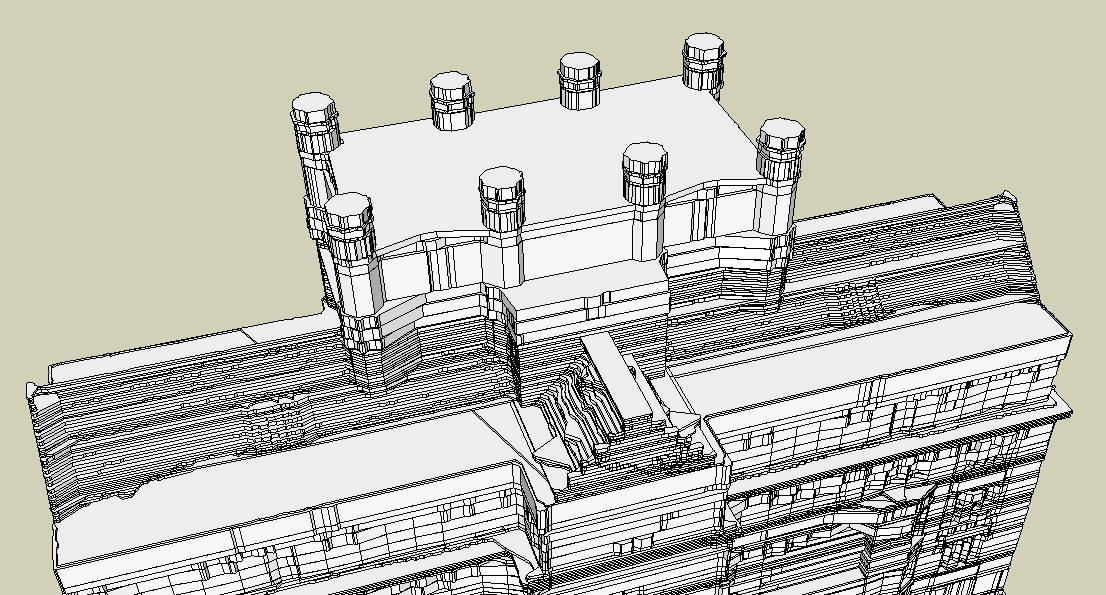
\includegraphics[width=0.7\textwidth]{extrude_1.png} \\
(a) \\
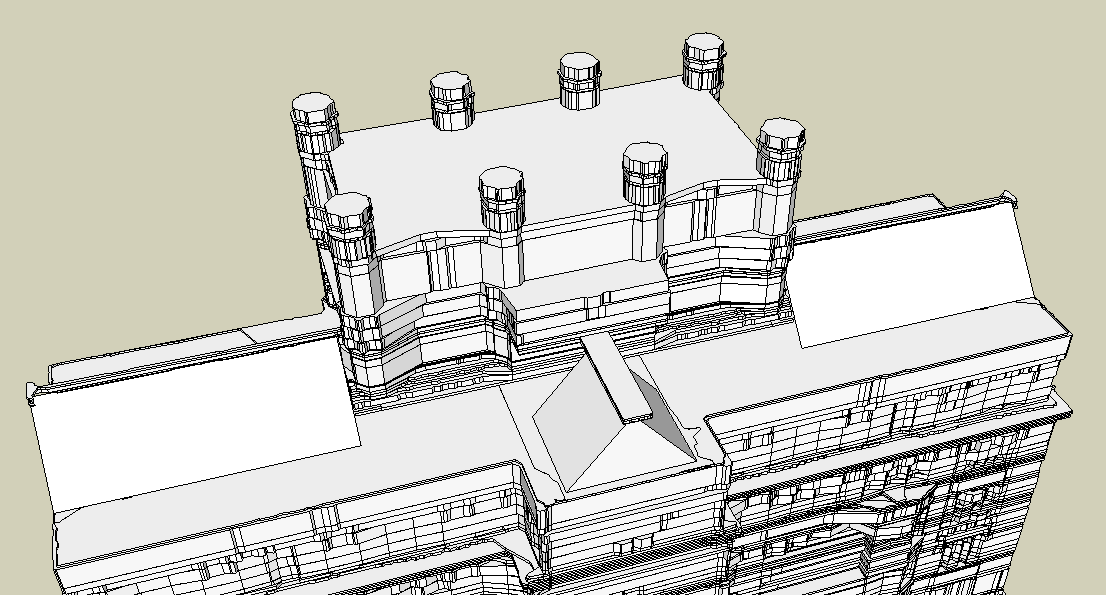
\includegraphics[width=0.7\textwidth]{extrude_2.png} \\
(b)
\end{tabular}
\end{center}
\caption{The top view of the 3D building shown (a) without tapered structures
and (b) with tapered structures.}
\label{fig:DXF_top}
\end{figure}

\section{Infering Taper Structure}
\label{sec:tsd}

The difficulty in inferring tapered structures is tied to the complexity of
the building structure itself.
Let's assume that the height range for the roof structure is
$H_R = [H_{lo}, H_{hi}]$.
If this is the only existing structure between $H_R$, it is simple and
straight-forward to detect and infer this part.
However, for some complicated structures, such as a mixed layout
of tapered and extruded structures, as depicted in \Fig{taper_seg},
some special treatment is needed to obtain the desired results.
Our approach is based on the divide-and-conquer strategy:
the whole structure $\boldsymbol{U}$ is segmented into independent
sub-structure units, $U_0, U_1, \ldots, U_N$.
Any sub-structure unit $U_i$ is constrained to contain a unique structure,
i.e., either a tapered or an extruded one.
Once each unit $U_i$ is inferred, the whole structure can be modeled by a
union operation of these sub-structures, i.e.,
$\boldsymbol{U} = \bigcup{U_i\{ i = 1,\ldots,N\}}$.
Before segmentation, the potential height ranges $H_R$ containing the tapered
structures must be computed.
This can be done by checking the frequency of the keyslice images.
The structure containing tapered sub-structures will show a wide and uniform
distribution of keyslice images.
This is a very useful clue for $H_R$ detection.

\begin{figure}[htbp]
\begin{center}
\begin{tabular}{c}
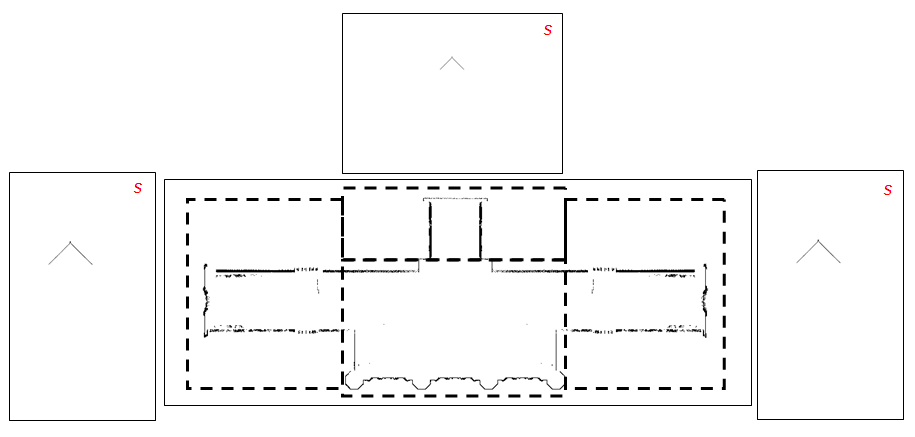
\includegraphics[width=0.8\textwidth]{extrude_3.png} \\
\end{tabular}
\end{center}
\caption{The top 2D slice of the 3D building. }
\label{fig:taper_seg}
\end{figure}

Once the potential height ranges $H_R$ is obtained, the next step is to
segment the whole structure $\boldsymbol{U}$ between $H_R$ into sub-structures,
$U_i, \; i = 0,\ldots,N$.
This is again done by applying the similarity measurement to sliced images
from orthogonal directions.
As before, the 3D data points inside the range of $H_R$ are projected
along both left-right ($X$ axis) and face-inside ($Z$ axis) directions.
Then, the keyslice detection is carried out based on the Hausdorff distance
similarity measurement for both directions.
These keyslices will segment the structure in $H_R$ into subunits of
$U_0, U_1, \ldots, U_N$.

For each subunit $U_i$, we must determine whether it represents an extruded or
a tapered structure.
This is done by checking in keyslice image $I_k$ of $U_i$ whether there exists
a pattern where two lines intersect with some appropriate angle.
If such a pattern exists in $I_k$, such as the images marked with red $s$ in
\Fig{taper_seg}, the unit $U_i$ is considered to be a tapered sub-structure unit.
Otherwise, $U_i$ is treated as an extruded sub-structure unit.
If $U_i$ is an extruded unit, its contours from the $y-$ axis are vectorized
and is ready for the union operation to obtain $\boldsymbol{U}$.
On the other hand, if $U_i$ is a tapered unit, the bottom and top position
have to be computed so that it can be reconstructed.
To do this, all line segments $\boldsymbol{L}$ in $U_i$ are computed using
the Hough Transform and the intersection point $P_0$ of $\boldsymbol{L}$
indicates the top position of the tapered unit.
The other end points $P_i$ of $\boldsymbol{L}$ are also computed to infer
the bottom shape and position. 
The model enhanced by taper operation is shown in \Fig{DXF_taper_model}.

\begin{figure}[htbp]
\begin{center}
\begin{tabular}{c}
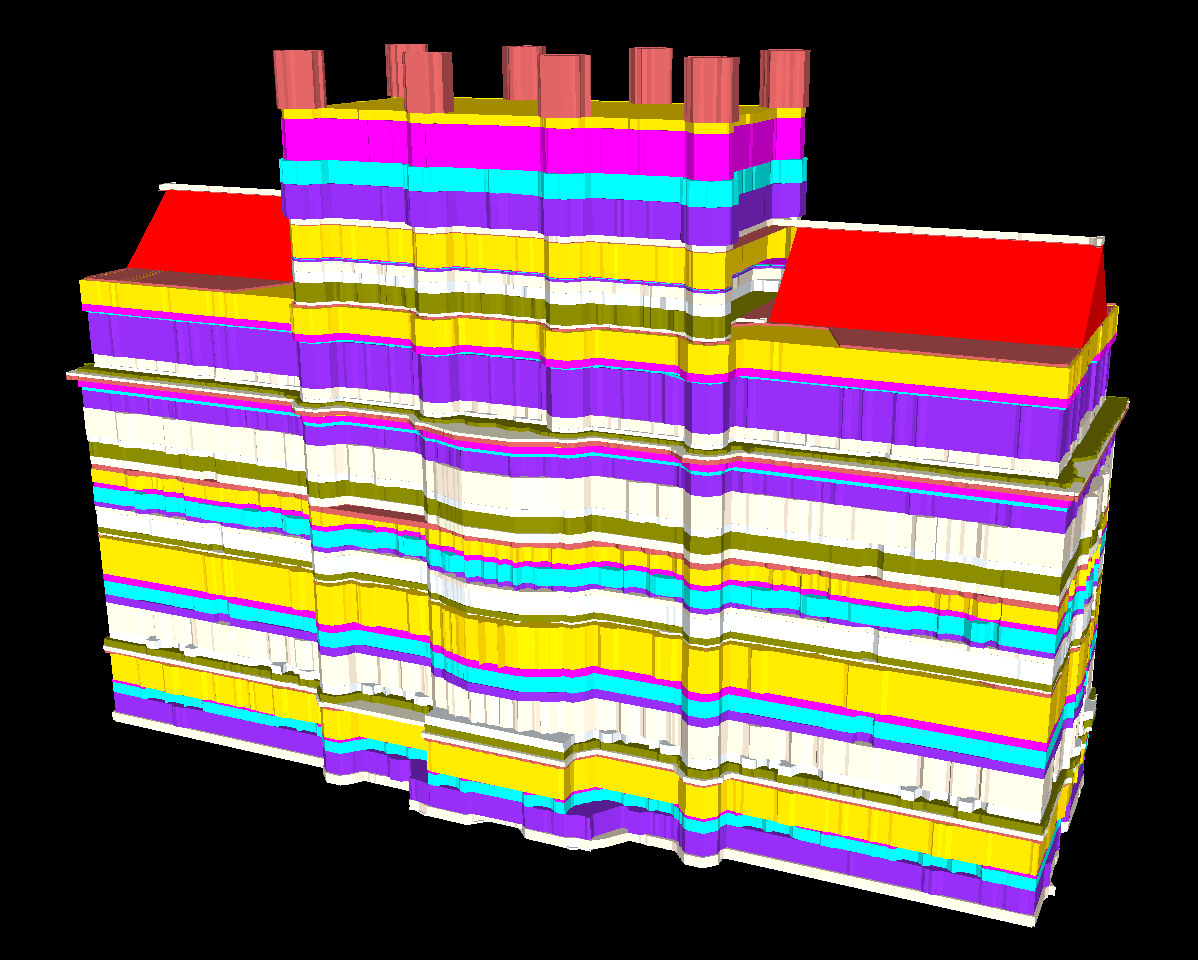
\includegraphics[width=0.8\textwidth]{taper_8_4.png}
\end{tabular}
\end{center}
\caption{ The reconstructed model enhanced by taper operation on roof structure. }
\label{fig:DXF_taper_model}
\end{figure}

\section{Taper-to-point Structure Inference}
\label{sec:tsd_ttp}
The approach we described and illustrated in the previous sections can only be
applied on the inference of taper-to-line structure. 
In addition to this, there is another
type of tapered structure, i.e. taper-to-point structure which appears frequently in 
Gothic architecture, such as churches.
Unlike the taper-to-line, this type of taper structures are not able to be inferred 
through the extruded structure from the orthogonal directions.
However, a nice characteristic of this type of taper structure is that
the vertices of the base geometry converge to a point, which is good clue for inference.
\Fig{DXF_taper_both} shows a synthetic data model consists of both taper-to-point (left)
and taper-to-line (right) structures. 

\begin{figure}[htbp]
\begin{center}
\begin{tabular}{c}
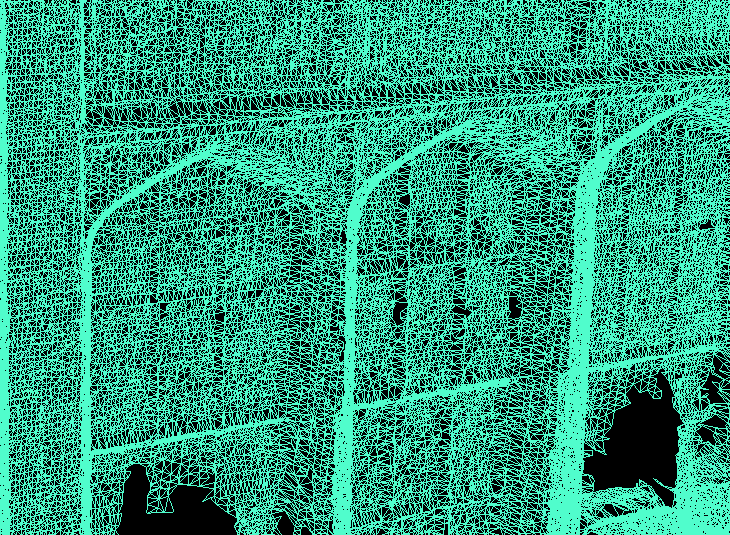
\includegraphics[width=0.8\textwidth]{BPA_TH.png}
\end{tabular}
\end{center}
\caption{ The synthetic model consists of taper-to-point and taper-to-line structures. }
\label{fig:DXF_taper_both}
\end{figure}

Without loss of generality, we assume that the sliced images of this special structure
can be vectorized by a closed polygon.
Let $S_i$, $S_j$ be two consecutive sliced images and $S_i$
has a smaller boundary than $S_j$. Based on this special structure, $S_i$ will be growing up
to cover $S_j$ by iterative dilation operations. By doing this, we can quickly locate the
bottom and top (a small region representing a point) slices of this special geometry
structure and therefore reconstruct this sub-model using these two slices.
The difference between this structure and the structure of tapering to a line is whether
$S_i$ and $S_j$ have any overlapping or common parts, which is easy to check.




